\documentclass[10pt, compress]{beamer}
\usetheme[titleprogressbar]{m}

\usepackage{booktabs}
\usepackage[scale=2]{ccicons}
\usepackage{minted}
\usepackage{dsfont}
\usepackage{caption}
\captionsetup[figure]{labelformat=empty}
\captionsetup{skip=0pt, belowskip=0pt}

\usepgfplotslibrary{dateplot}

\usemintedstyle{trac}

\title{Poisson Processes and 911 Calls}
\subtitle{}
\date{\today}
\author{Jacob Mortensen}
\institute{Brigham Young University}

\begin{document}
  \maketitle
  
  \section{Introduction}
  \begin{frame}
    \frametitle{Introduction}
    \begin{itemize}
      \item Extreme heat scenarios pose a significant threat to public health
      \item It is of interest for researchers to understand how the effect of heat varies by location
    \end{itemize}
  \end{frame}
  \begin{frame}
    \frametitle{Introduction}
    \centering
    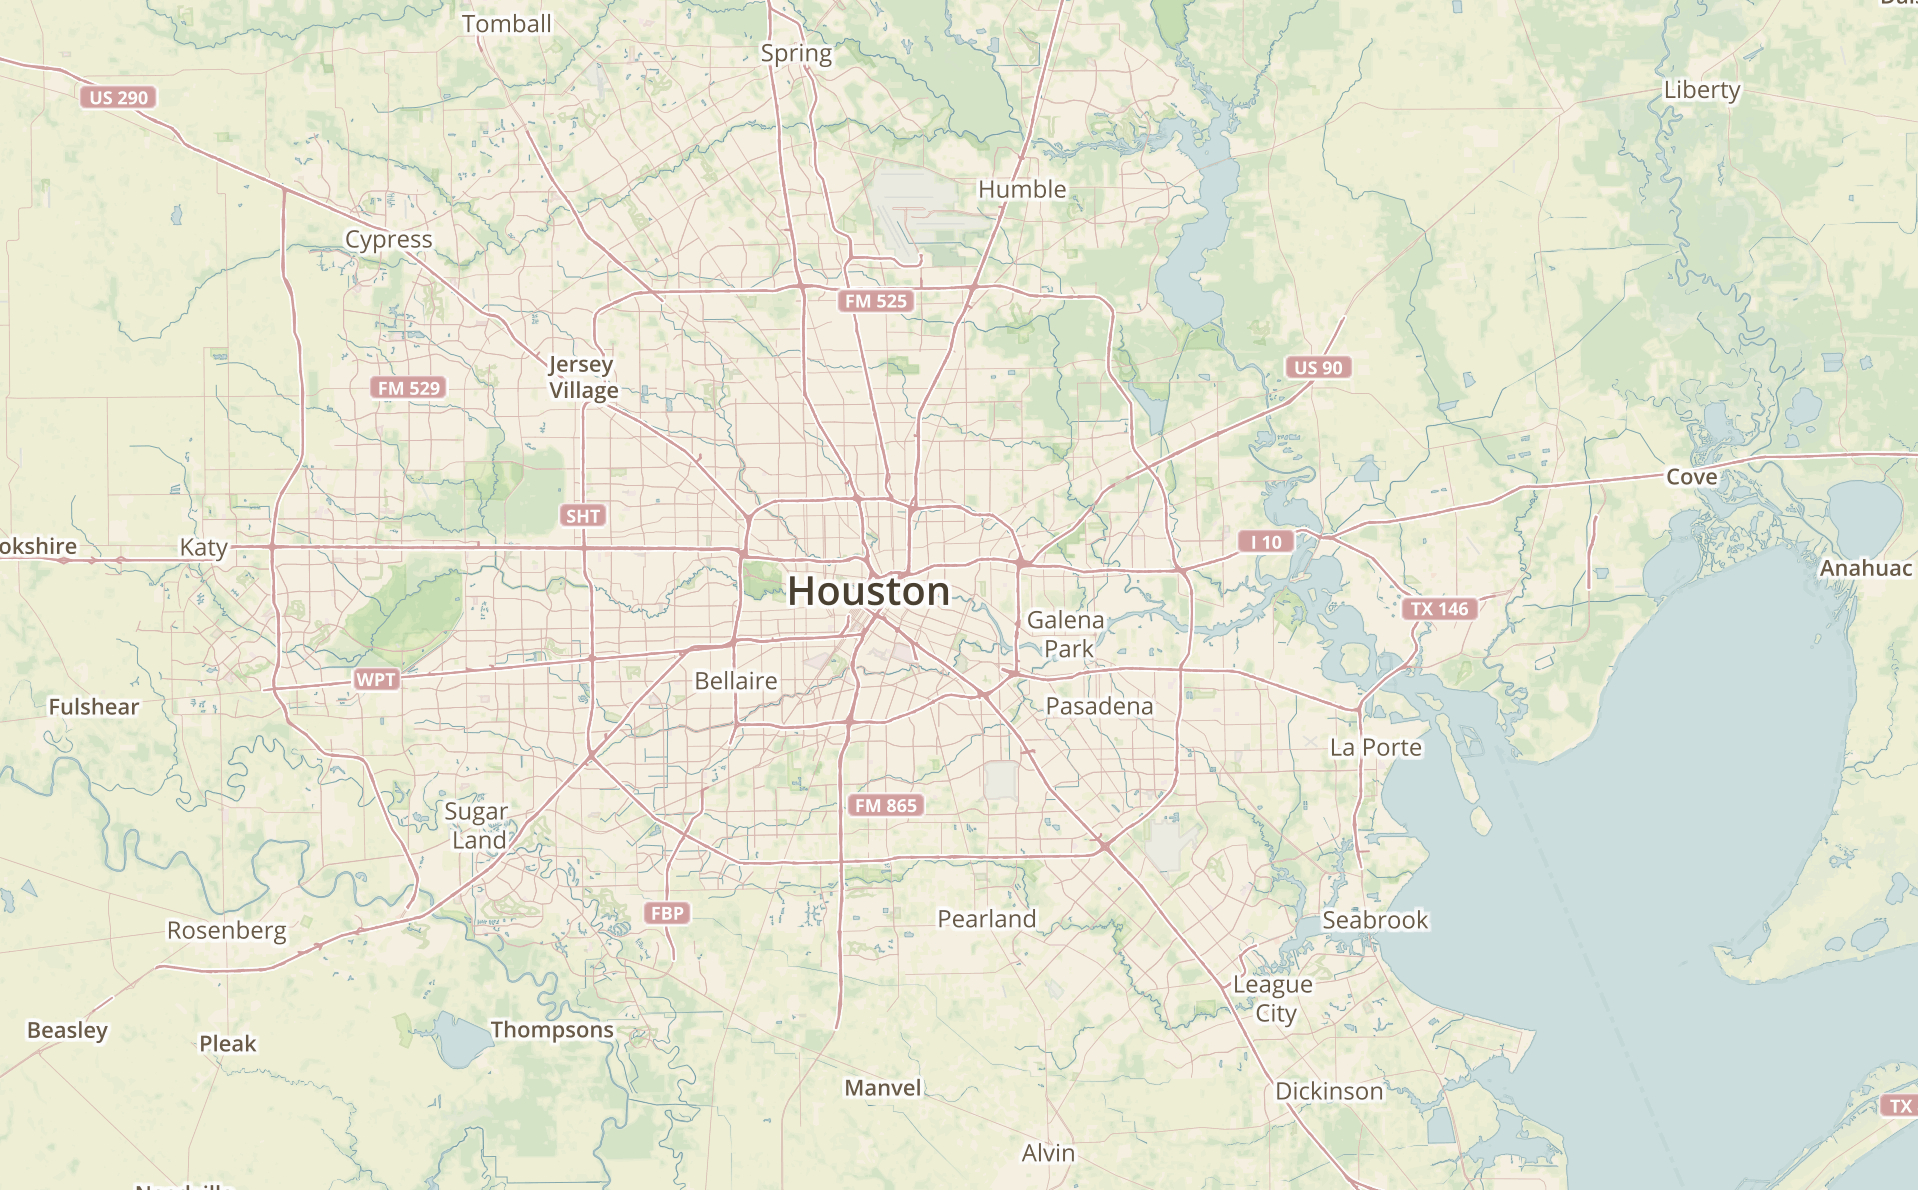
\includegraphics[width=0.8\textwidth]{houston_map.jpg}
  \end{frame}
  \begin{frame}{Introduction}
    Our data includes information about 1389 heat-related 911 calls \newline
    \newline
    How many 911 calls will come in and where they will come from? \newline

    \centering
    \begin{minipage}{0.8\textwidth}
      Spatial data is:
      \begin{itemize}
        \item nonlinear
        \item highly correlated
      \end{itemize}
    so how do we model it?
    \end{minipage}
  \end{frame}
  \begin{frame}
    \frametitle{Point Process Models}
    We use a point process model
    \begin{itemize}
      \item Models both frequency and location of events
      \item Relies on an intensity function, $\Lambda(x)$
      \item $\Lambda(x)$ integrates to the expected number of events
      \item If we normalize $\Lambda(x)$ it becomes the density of event location
    \end{itemize} 
    $\Lambda(x)$ is the key!
  \end{frame}

  \section{Model}
  \begin{frame}
    \frametitle{Model}
      \begin{itemize}
        \item $\mathbf{s_1}, \mathbf{s_2}, \dots, \mathbf{s_N}$ where N = 1389 are the latitude-longitude coordinates of the observed 911 calls
        \item $\mathcal{S}$ is the set of all latitude-longitude coordinates in Houston
        \item $N \sim Pois(\int_{\mathcal{S}} \Lambda(s))$
        \item $f(\mathbf{s_1}, \mathbf{s_2}, \dots, \mathbf{s_N}|N) = \prod_{i=1}^{N} \frac{\Lambda(\mathbf{s_i})}{\int_{\mathcal{S}}\Lambda(\mathbf{s})}$ 
      \end{itemize}
  \end{frame}
  \begin{frame}
    \frametitle{Model}
    Our likelihood is:
      $$L(\Lambda(\mathbf{s})) = \frac{\exp(-\int_{\mathcal{S}}\Lambda(\mathbf{s}))\left(\int_{\mathcal{S}}\Lambda(\mathbf{s})\right)^{N}}{N!}
        \prod_{i=1}^{N}\frac{\Lambda(\mathbf{s_i})}{\int_{\mathcal{S}}\Lambda(\mathbf{s})}$$
    which is equivalent to:
      $$L(\Lambda(\mathbf{s})) = \exp\left(-\int_{\mathcal{S}}\Lambda(\mathbf{s})\right) \prod_{i=1}^{N}\Lambda(\mathbf{s}_i)$$
  \end{frame}
  \begin{frame}
    \frametitle{Model}
    \begin{itemize}
      \item To simplify we are going to divide $\mathcal{S}$ into a grid
      \item $\mathbf{s_1}^{*}, \mathbf{s_2}^{*}, \dots, \mathbf{s_K}^{*}$ where K = 1428 are the latitude-longitude coordinates of the  prediction locations
      \item This allows us to discretize $\Lambda(\mathbf{s})$ to make modeling easier:
    \end{itemize}
        $$ \Lambda(\mathbf{s}) = \delta \sum_{k=1}^K \frac{\lambda_k}{|\mathcal{G}_k|} \mathds{1} \left\{ \mathbf{s} \in \mathcal{G}_k \right\} $$
  \end{frame}
  \begin{frame}
    \frametitle{Model}
    $$ \Lambda(\mathbf{s}) = \delta \sum_{k=1}^K \frac{\lambda_k}{|\mathcal{G}_k|} \mathds{1} \left\{ \mathbf{s} \in \mathcal{G}_k \right\} $$
    \begin{itemize}
      \item $\delta$ is the expected number of 911 calls
      \item $\lambda_k$ is the probability that a 911 call occurs in grid cell $\mathcal{G}_k$
      \item $\mathcal{G}_k$ is the set of spatial coordinates that are closest to grid point $\mathbf{s}_k^{*}$
      \item $|\mathcal{G}_k| = \int_{\mathcal{G}_k}d\mathbf{s}$ is the the ``area" of grid cell $\mathcal{G}_k$
      \item $\lambda_k \in (0,1)$ and $\sum_{k=1}^K \lambda_k = 1$
    \end{itemize}
  \end{frame}
  \begin{frame}
    \frametitle{Model}
    \centering
    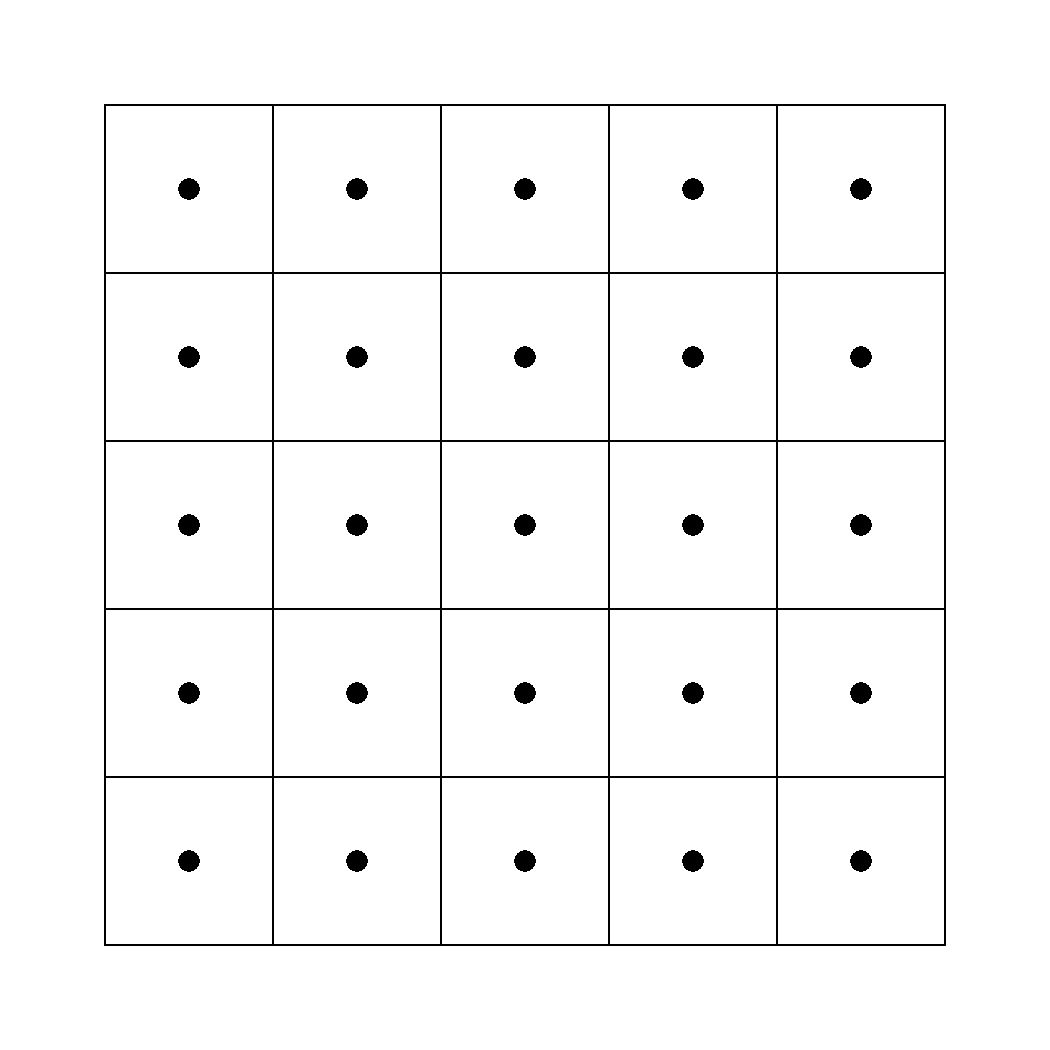
\includegraphics[height=0.8\textheight]{blank_grid.pdf}
  \end{frame}
  \begin{frame}
    \frametitle{Model}
    \centering
    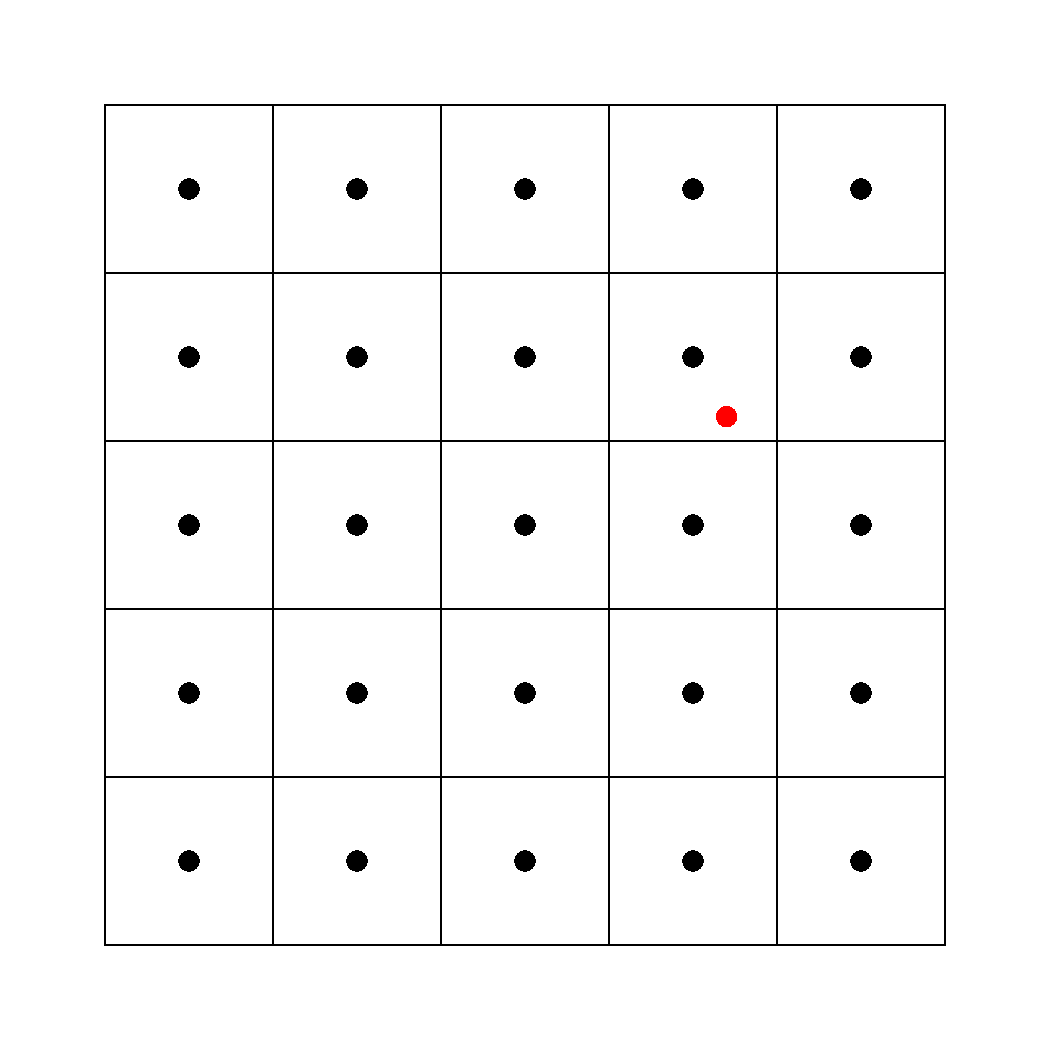
\includegraphics[height=0.8\textheight]{grid_spot.pdf}
  \end{frame}
  \begin{frame}
    \frametitle{Model}
    \centering
    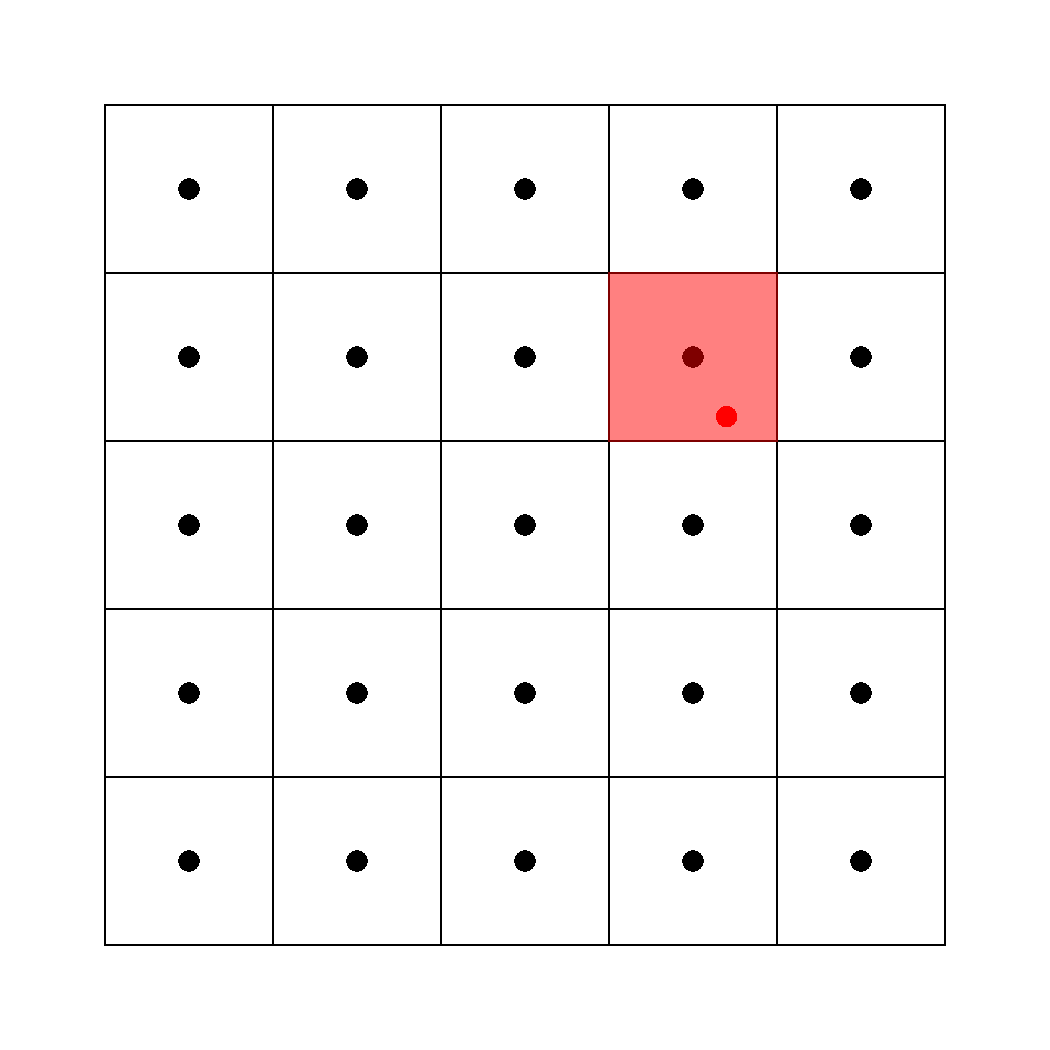
\includegraphics[height=0.8\textheight]{grid_spot_highlighted.pdf}
  \end{frame}
  \begin{frame}
    \frametitle{Model}
    With $\Lambda(\mathbf{s}) = \delta \sum_{k=1}^K \frac{\lambda_k}{|\mathcal{G}_k|} \mathds{1} \left\{ \mathbf{s} \in \mathcal{G}_k \right\}$ our likelihood can be written
    $$L(\Lambda(\mathbf{s})) = \exp\left(-\delta\right) \delta^N \prod_{i=1}^{N}\frac{\lambda_{\left\{k: \mathbf{s_i} \in \mathcal{G}_k \right\}}}{|\mathcal{G}_k|}$$   
  \end{frame}
  \section{Fitting the Model}
  \begin{frame}
    \frametitle{Fitting the Model}
      If we use a gamma($0.001, 0.001$) distribution as the prior for $\delta$ 
      then 
    $$ \pi(\delta)L(\delta|N) \propto \exp(-1.001\delta)\delta^{N+0.001-1}$$
    which we recognize as the kernel of a gamma($N+0.001, 1.001$) distribution
  \end{frame}
  \begin{frame}
    \frametitle{Fitting the Model}
    How can we use the spatial smoothness in $\Lambda(\mathbf{s})$ to estimate $\lambda_1, \dots, \lambda_k$?
    \pause
    \newline
    \newline
    We use a Gaussian process:
    \begin{itemize}
      \item Let $\lambda_k \propto \exp(\lambda_k^{*})$
      \item Let $\boldsymbol{\lambda}^{*} = \begin{pmatrix} \lambda_1^{*} \\ \vdots \\ \lambda_k^{*} \end{pmatrix} \sim \mathcal{N}(\mathbf{0}, \sigma^2\mathbf{M})$
      \item $\mathbf{M}$ is a $K \times K$ correlation matrix with $ij^{th}$ element $M_{\nu}(\|\mathbf{s}_i^{*}-\mathbf{s}_j^{*}\|~| \phi)$ where $M_{\nu}(d | \phi)$
            is the Mat\'{e}rn correlation function with smoothness $\nu$ and decay $\phi$
      \item Then it follows that $\lambda_k = \frac{\exp(\lambda_k^{*})}{\sum_{j=1}^{K}\exp(\lambda_j^{*})}$

    \end{itemize}
  \end{frame}
  \begin{frame}
    \frametitle{Fitting the Model}
    If we use an inverse-gamma($0.01$, $0.01$) distribution as the prior for $\sigma^2$ then 
    $$ \pi(\sigma^2)L(\sigma^2|\boldsymbol\lambda^{*}) \propto 
      (\sigma^2)^{-(0.01+\frac{N}{2})}\exp\left\{-\frac{1}{2\sigma^2}\left[0.01+\frac{1}{2}(\boldsymbol\lambda^{*})^{'}\mathbf{M}^{-1}(\boldsymbol\lambda^{*})\right]\right\}
    $$
    which we recognize as the kernel of an inverse-gamma$(0.01+\frac{N}{2}, 0.01+\frac{1}{2}(\boldsymbol\lambda^{*})^{'}\mathbf{M}^{-1}(\boldsymbol\lambda^{*}))$
    distribution
  \end{frame}
  \begin{frame}
    \frametitle{Fitting the Model}
      With $\boldsymbol\lambda^{*} \sim \mathcal{N}(0, \sigma^2\mathbf{M})$, 
    $$ \pi(\boldsymbol\lambda^{*})L(\boldsymbol\lambda^{*} | N) \propto 
      \exp\left(-\frac{1}{2\sigma^2}(\boldsymbol\lambda^{*})^{'}\mathbf{M}^{-1}(\boldsymbol\lambda^{*})\right)\prod_{k=1}^{K}\lambda_k^{N_k} $$
  \end{frame}
  \begin{frame}
    \frametitle{Fitting the Model}
    Using a Metropolis within Gibbs sampler, we generate 100,000 draws for $\boldsymbol\lambda^{*}$, $\delta$ and $\sigma^2$
    \begin{figure}
      \begin{minipage}{0.3\textwidth}
        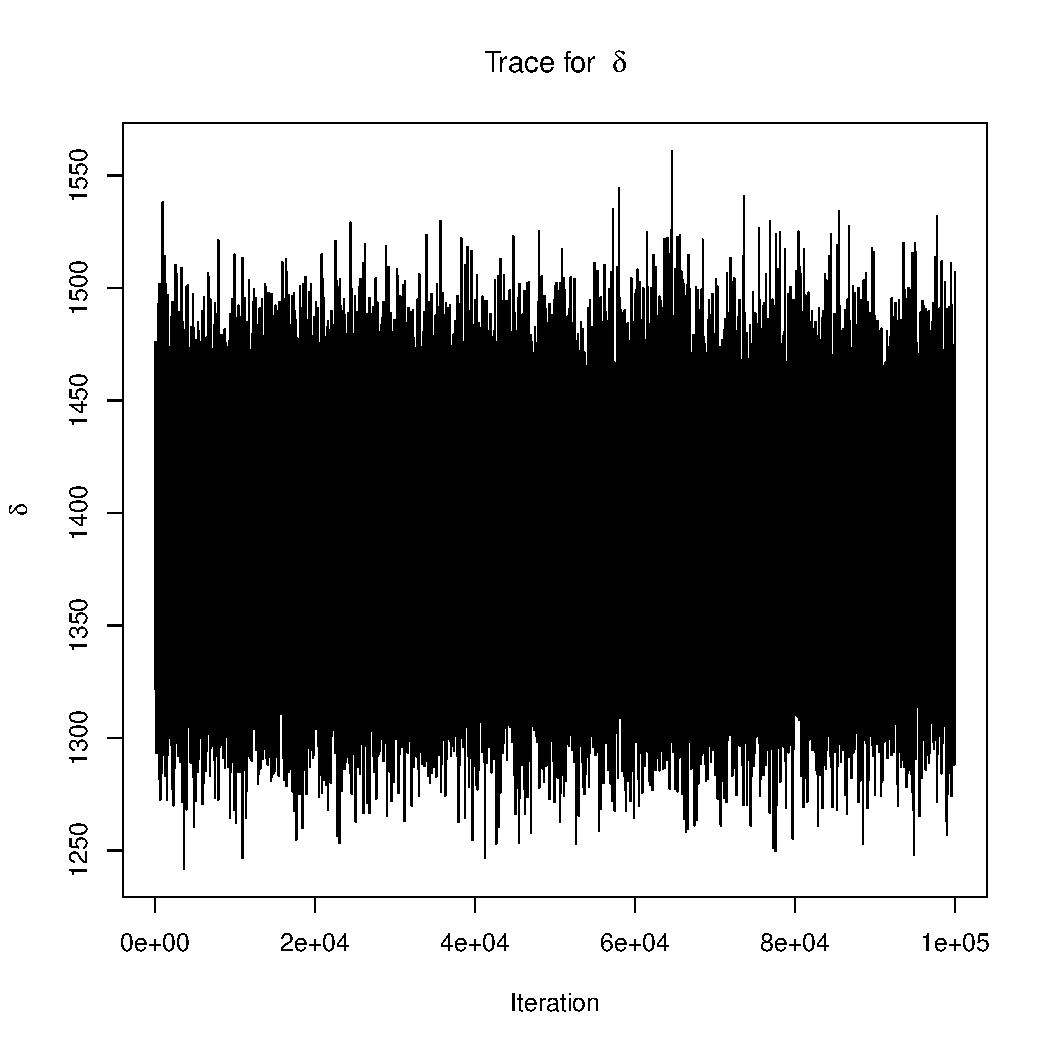
\includegraphics[width=1.0\textwidth]{delta_trace.pdf}
        \caption{Trace for $\delta$}
      \end{minipage}
      \hfill
      \begin{minipage}{0.3\textwidth}
        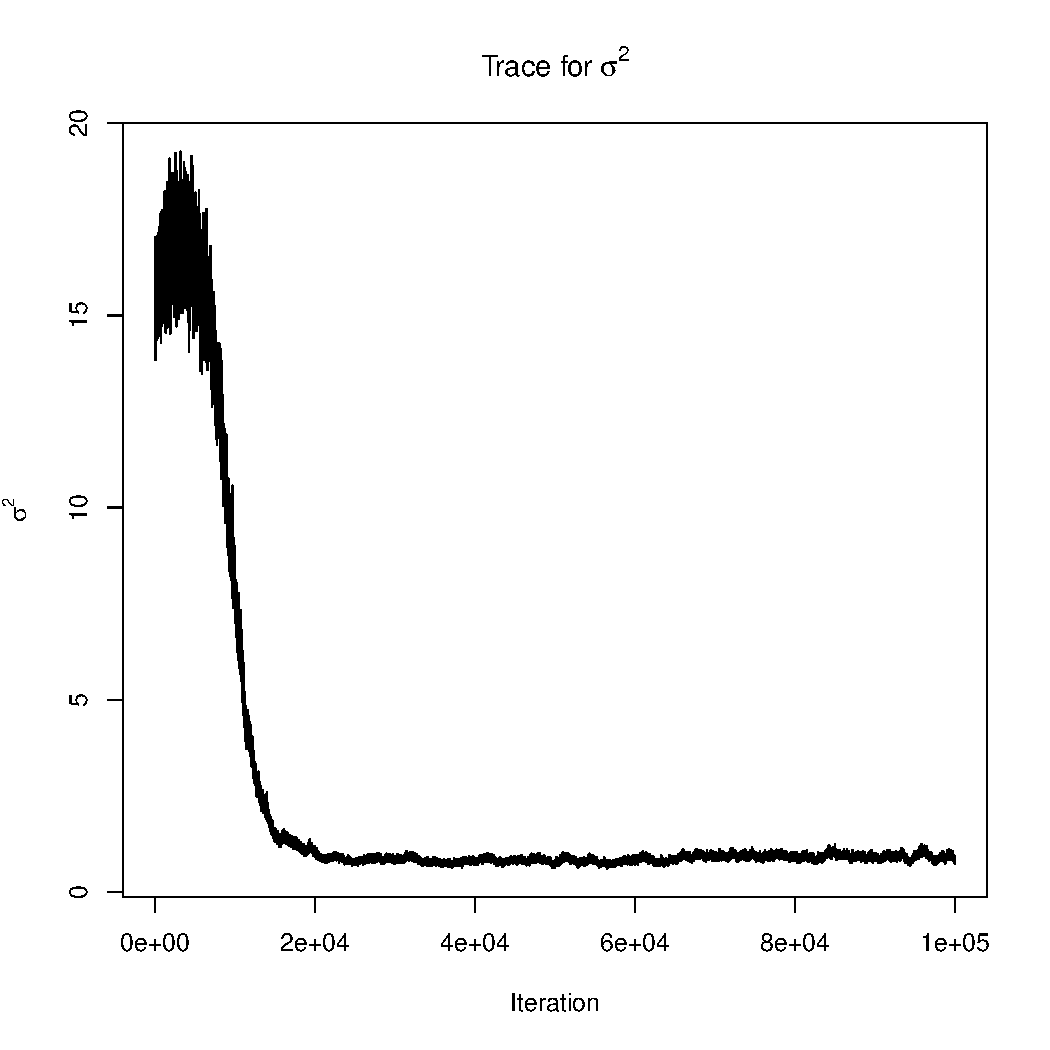
\includegraphics[width=1.0\textwidth]{sigma_trace.pdf}
        \caption{Trace for $\sigma^2$}
      \end{minipage}
      \hfill
      \begin{minipage}{0.3\textwidth}
        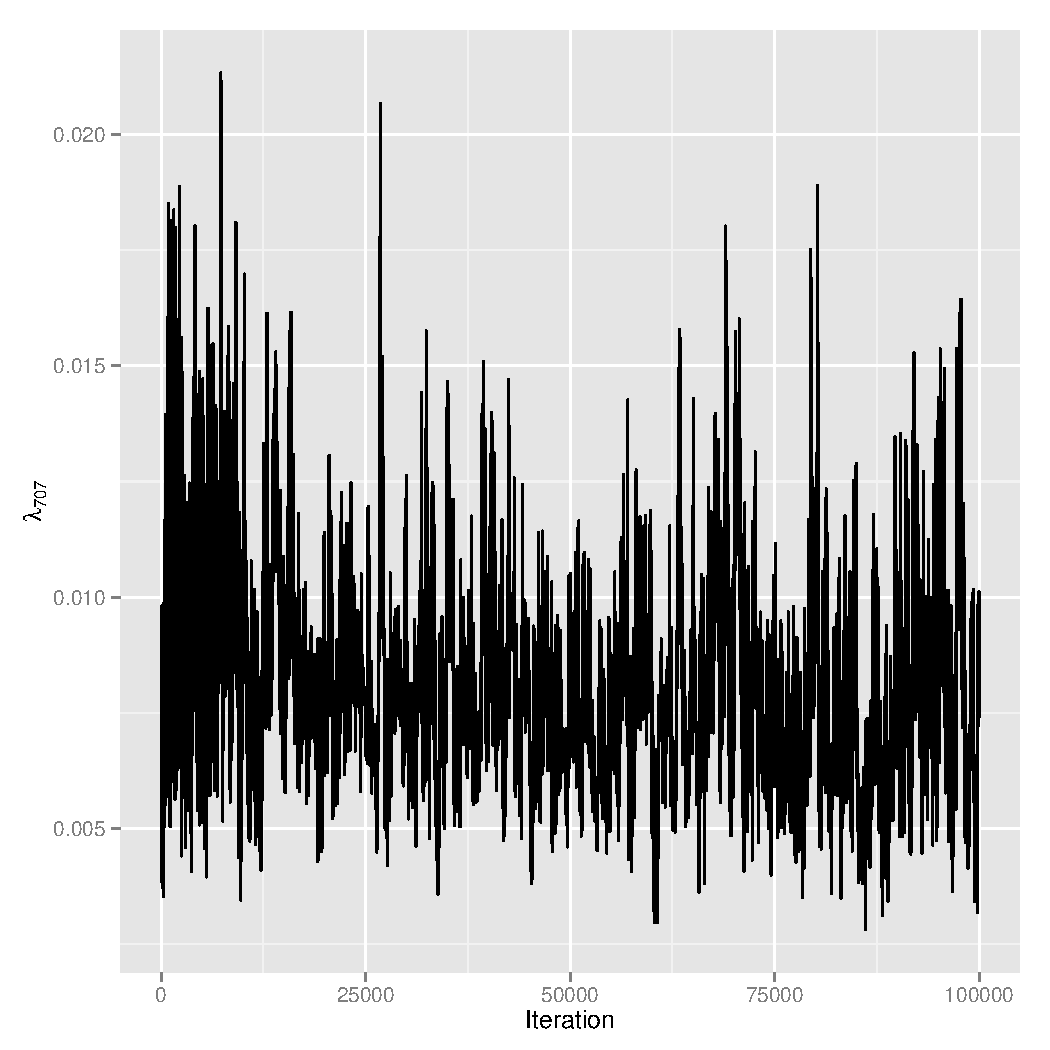
\includegraphics[width=1.0\textwidth]{lambda_trace.pdf}
        \caption{Trace for $\lambda_{707}$}
      \end{minipage}
    \end{figure}
  \end{frame}
  \section{Results}
  \begin{frame}
    \frametitle{Results}
    \centering
    \begin{figure}
      \caption{Posterior Density of $\delta$}
      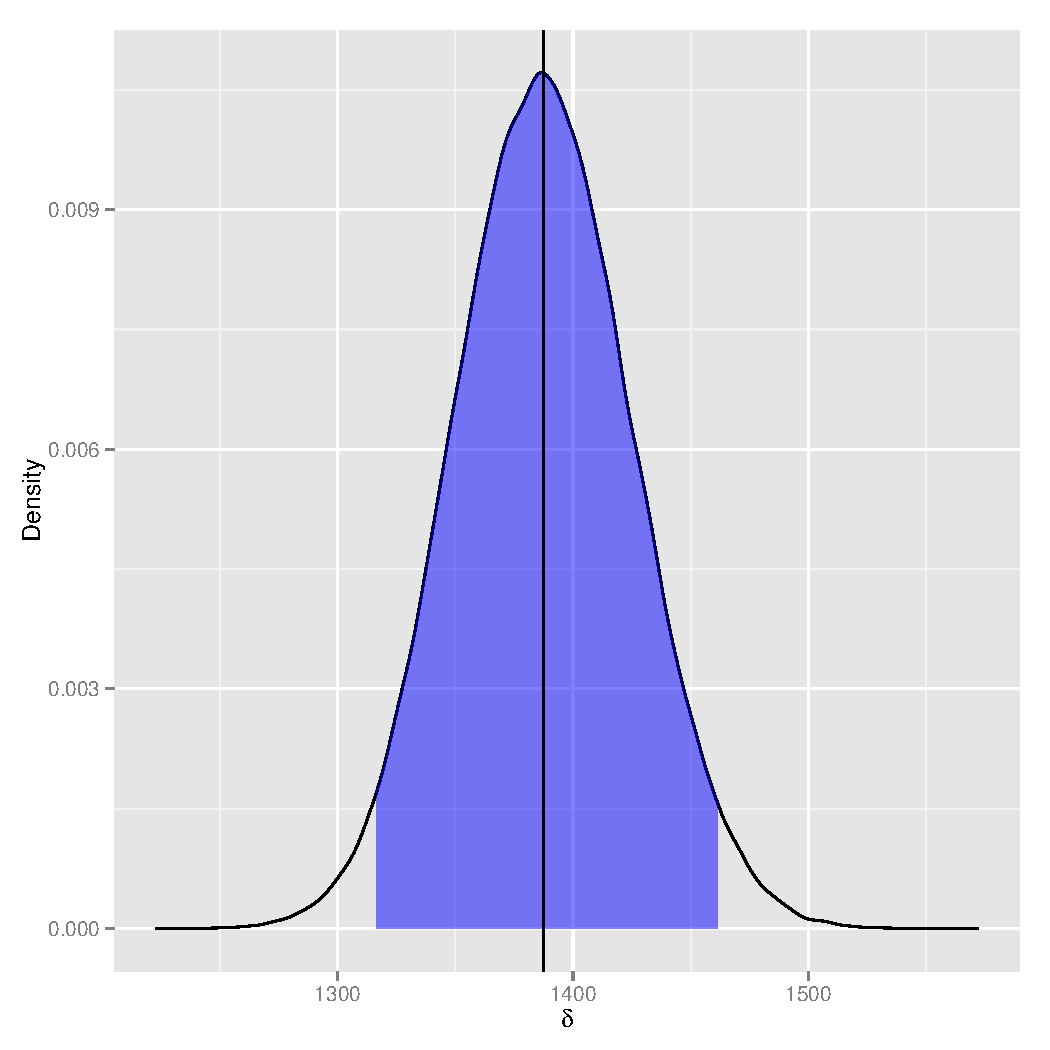
\includegraphics[height=0.625\textheight]{delta_density.pdf}
    \end{figure}
    Posterior Mean: 1387.65
  \end{frame}
  \begin{frame}
    \frametitle{Results}
    \centering
    \begin{figure}
      \caption{Posterior Density of $\sigma^2$}
      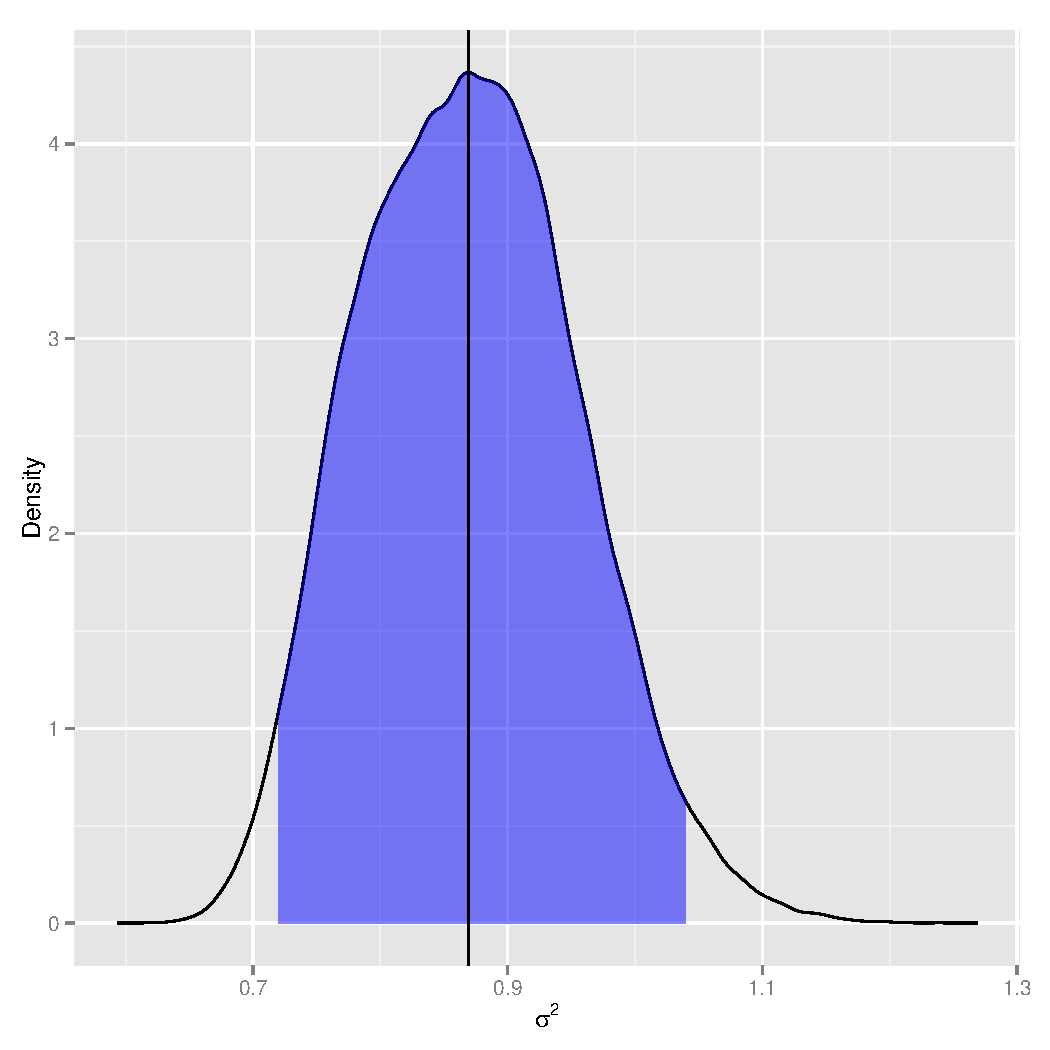
\includegraphics[height=0.625\textheight]{s2_density.pdf}
    \end{figure}
    Posterior Mean: 0.87
  \end{frame}
  \begin{frame}
    \frametitle{Results}
   \centering
    \begin{figure}
      \caption{Posterior Density of $\boldsymbol\lambda$}
      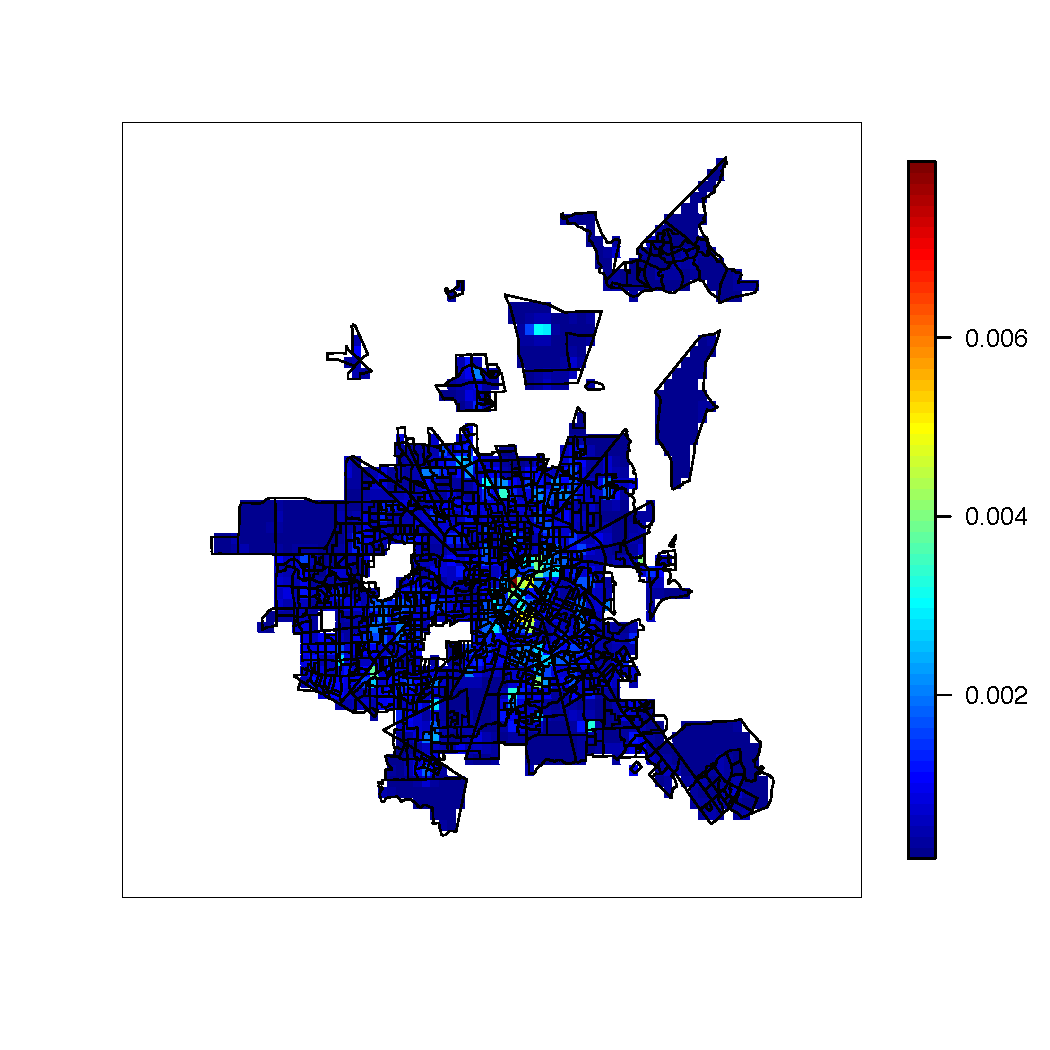
\includegraphics[height=0.7\textheight]{posteriorLocationDensity.pdf}
    \end{figure}
  \end{frame}
  \section{Questions?}
\end{document}
